\newpage
\section{Resultados}

\subsection{Modulador série}

\subsubsection{Sinal de saída}
Após a simulação, obtemos a forma de onda mostrada na figura \ref{f_saida_serie}, com o potenciômetro na posição 0, ou seja, com o máximo índice de modulação.

\begin{figure}[H]
    \centering
    \caption{Onda de saída para o modulador série.}
    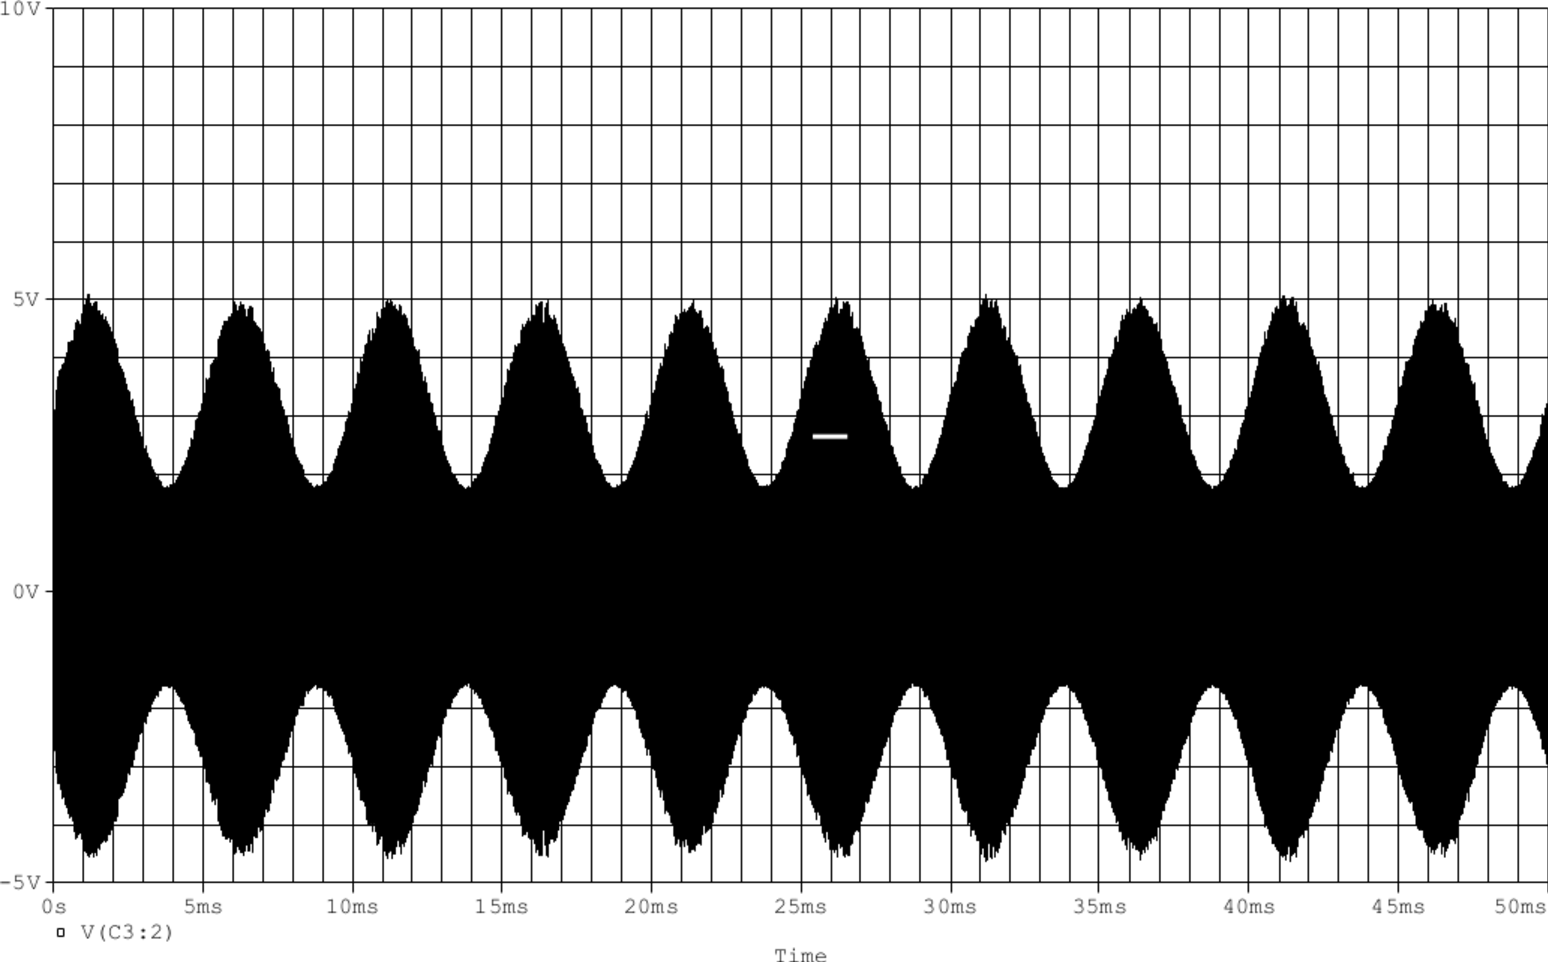
\includegraphics[scale=0.4]{Imagens/saida_serie.pdf}
    \label{f_saida_serie}
\end{figure}

Para um índice de modulação maior que 1, foi necessário aumentar a tensão do sinal modulante para 4.5$V_p$. Dessa forma, obtivemos o sinal de saída da figura \ref{f_saida_serie_gamma_ge_1}.

\begin{figure}[H]
    \centering
    \caption{Onda de saída para o modulador série com $\gamma \ge 1$.}
    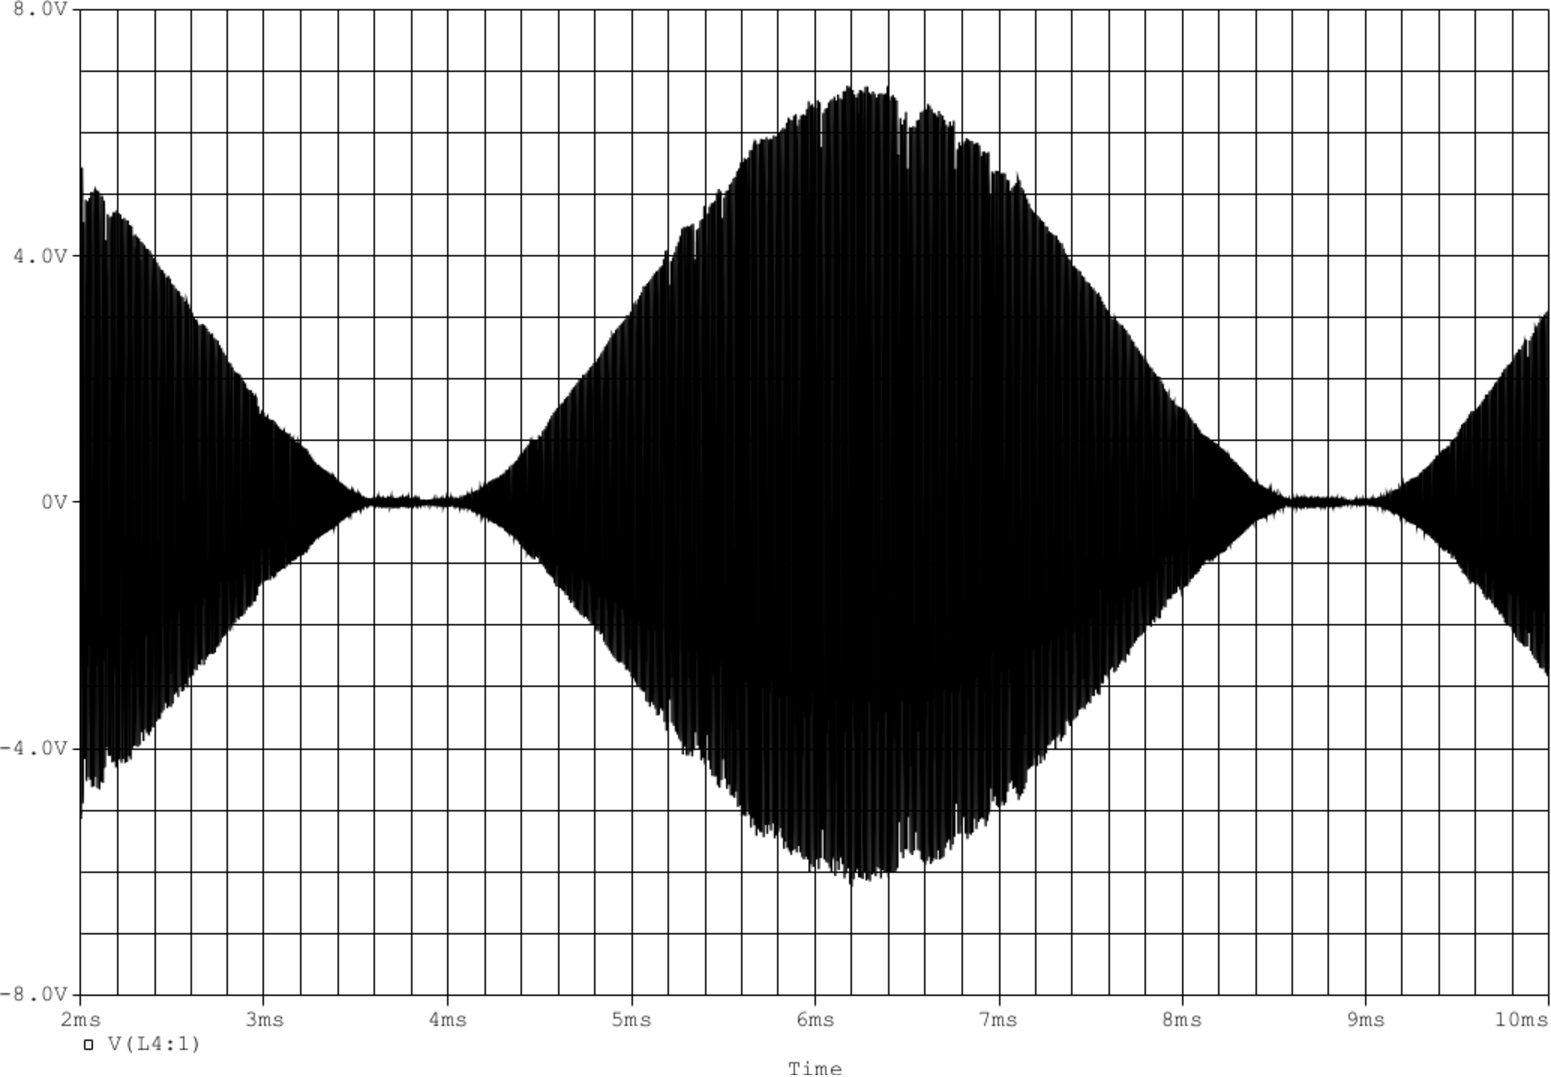
\includegraphics[scale=0.4]{Imagens/saida_serie_gamma_ge_1.pdf}
    \label{f_saida_serie_gamma_ge_1}
\end{figure}

\subsubsection{Índice de modulação}
Através do método 1, o valor de $\gamma$ calculado foi de 
\[ 
\gamma_1 = \frac{4.4988-1.7184}{4.4988+1.7184} = 0.4472.
\]

Mudando o eixo X do gráfico para o sinal modulante, obtivemos a imagem da figura \ref{f_trapezio_serie}, de onde foi possível calcular
\[
\gamma_2 = \frac{8.2133-3.4907}{8.2133+3.4907} = 0.4435
\]

Como podemos observar, os dois métodos deram resultados bastante próximos.
O desvio observado se deve ao fato da dificuldade em se obter uma medida precisa no gráfico do trapézio.

\begin{figure}[H]
	\centering
    \caption{Método do trapézio para o modulador série com $\gamma \le 1$.}
	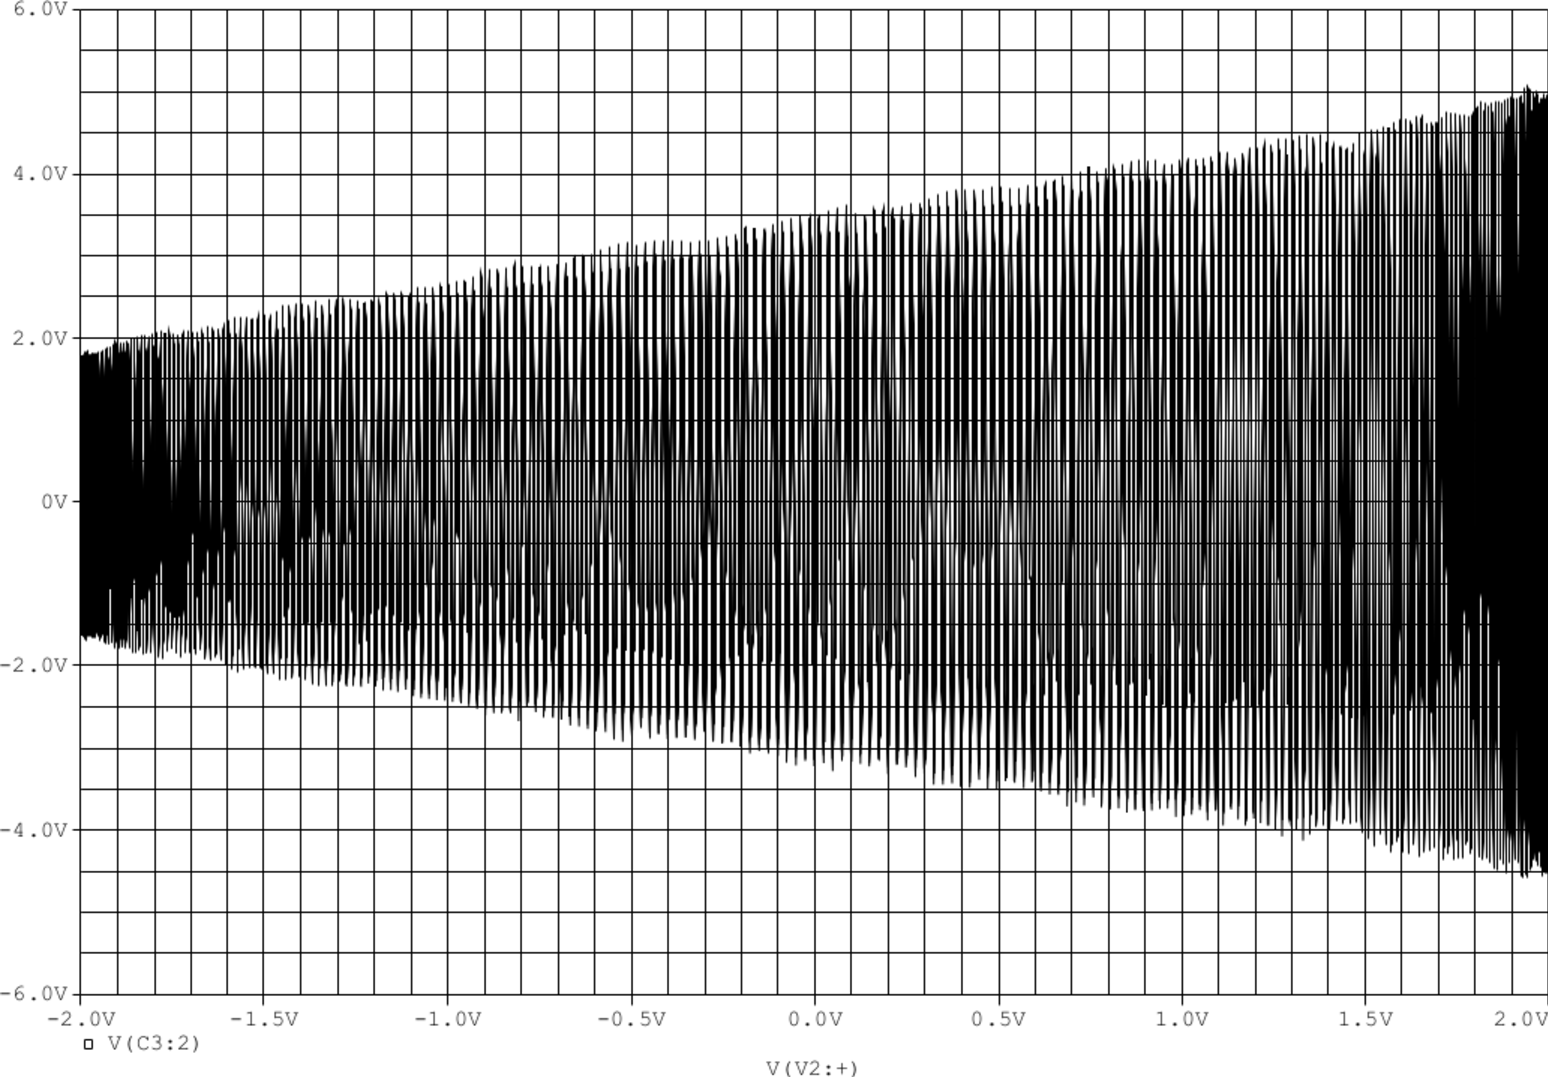
\includegraphics[scale=0.4]{Imagens/trapezio_serie.pdf}
	\label{f_trapezio_serie}
\end{figure}

Para $\gamma > 1$, o método do trapézio resultou na imagem da figura \ref{f_trapezio_gamma_ge_1}. É possível observar a não linearidade das amplitudes na curva. Sendo assim, o método do trapézio não é valido para moduladores com índice de modulação maior que 1.

\begin{figure}[H]
    \centering
    \caption{Método do trapézio para o modulador série com $\gamma > 1$.}
    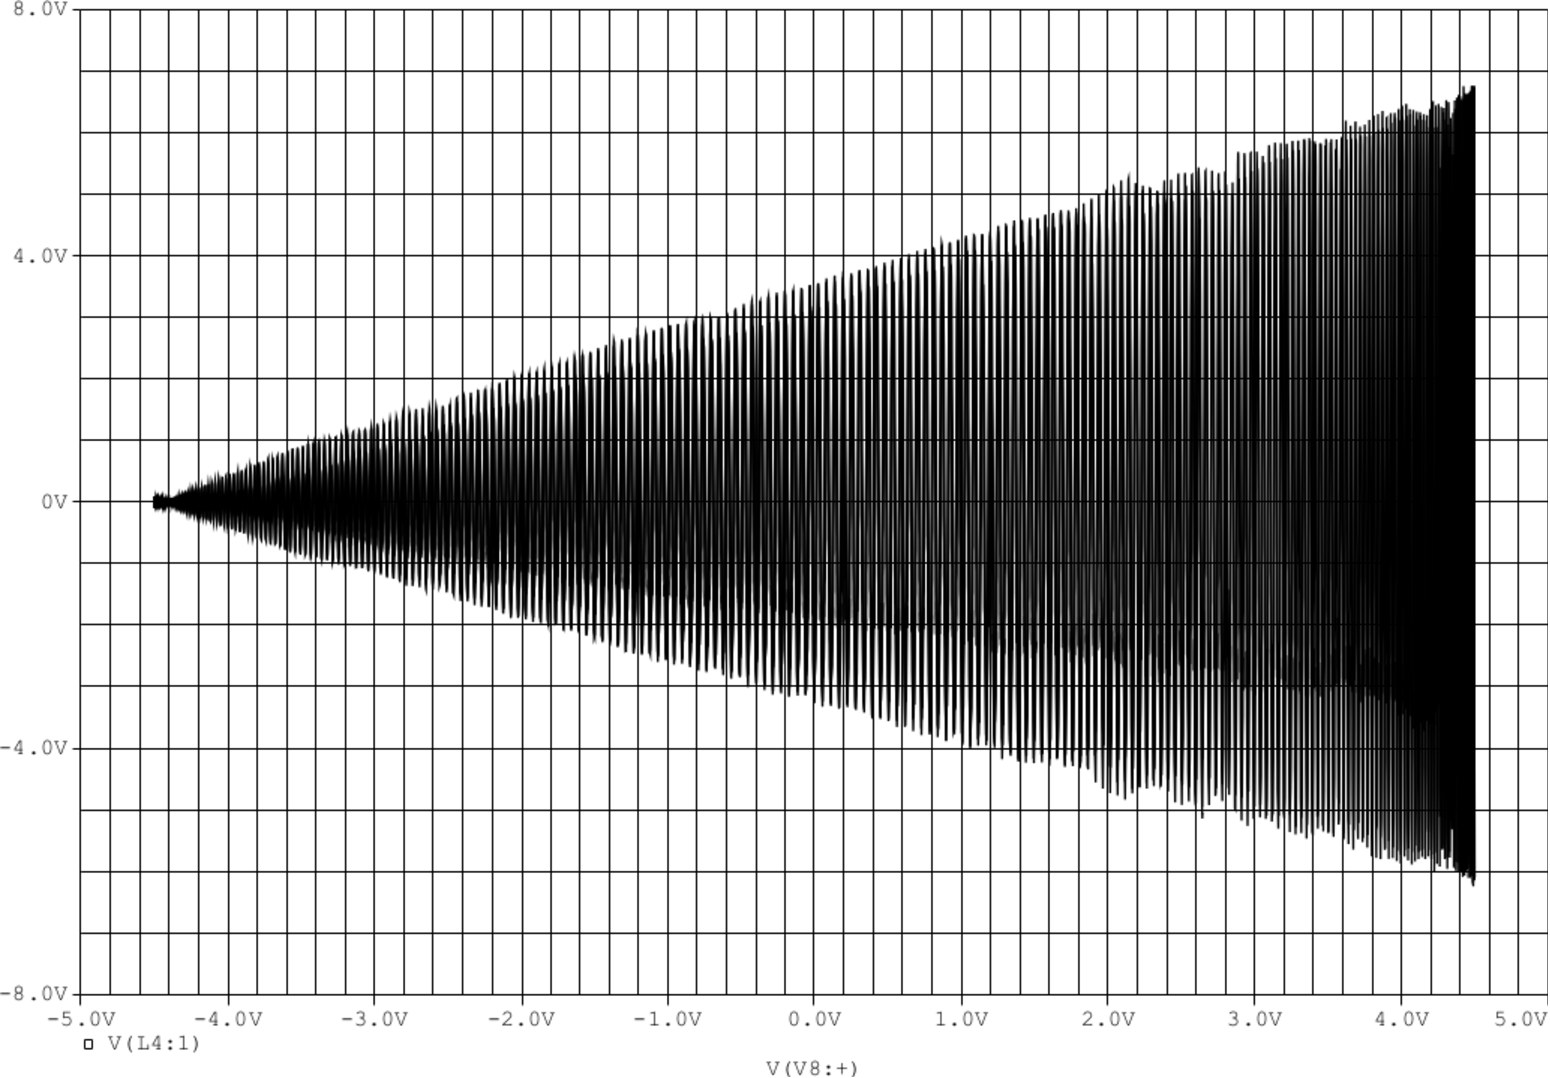
\includegraphics[scale=0.4]{Imagens/trapezio_gamma_ge_1.pdf}
    \label{f_trapezio_gamma_ge_1}
\end{figure}

\subsubsection{Espectro}

O espectro do sinal modulado da figura \ref{f_saida_serie} é apresentado na figura \ref{f_fft_serie}.
Podemos observar a portadora (com maior energia) na frequência $f_c = 100kHz$ e as raias laterais em $f_c \pm 2$, características do modulador AM/DSB.

\begin{figure}[H]
    \centering
    \caption{Espectro do sinal da figura \ref{f_saida_serie}.}
    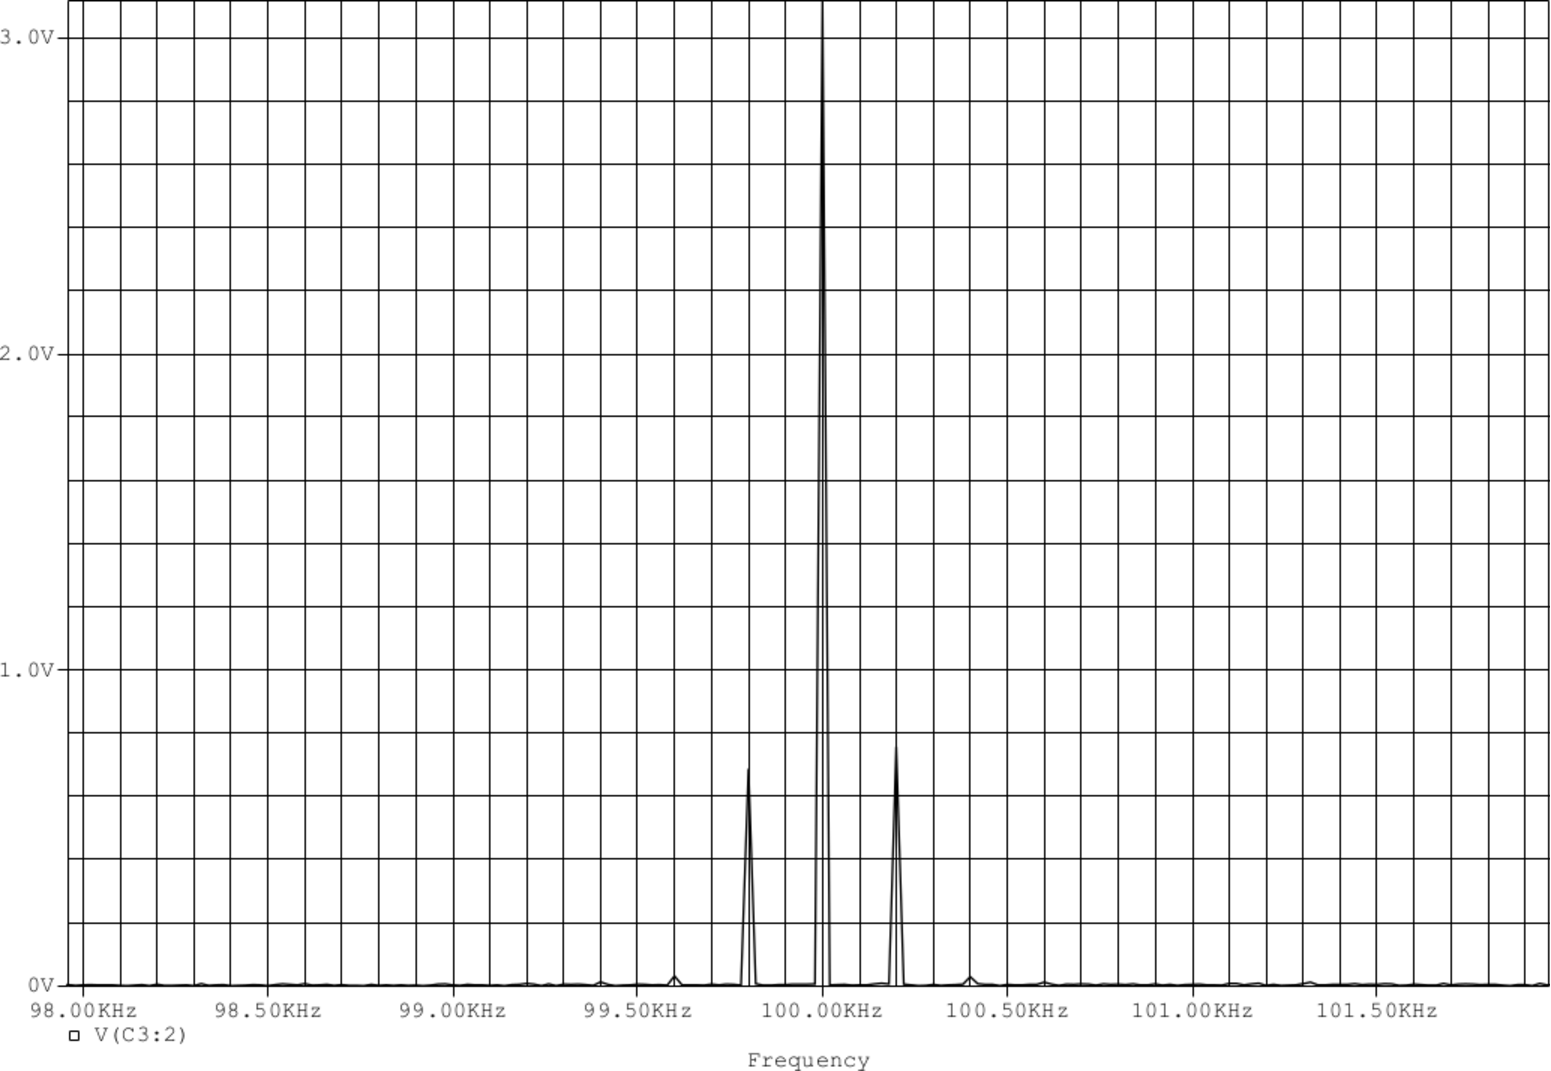
\includegraphics[scale=0.4]{Imagens/fft_serie.pdf}
    \label{f_fft_serie}
\end{figure}

\subsubsection{Fator de mérito}

Para o calculo do fator de mérito do circuito, o sinal modulante foi substituído por uma fonte do tipo $V_{ac}$ e foi realizada uma simulação do tipo varredura em frequência (\textit{Frequency Sweep}), resultando no gráfico da figura \ref{f_q_serie}.

\begin{figure}[H]
    \centering
    \caption{Resposta em frequência do modulador série.}
    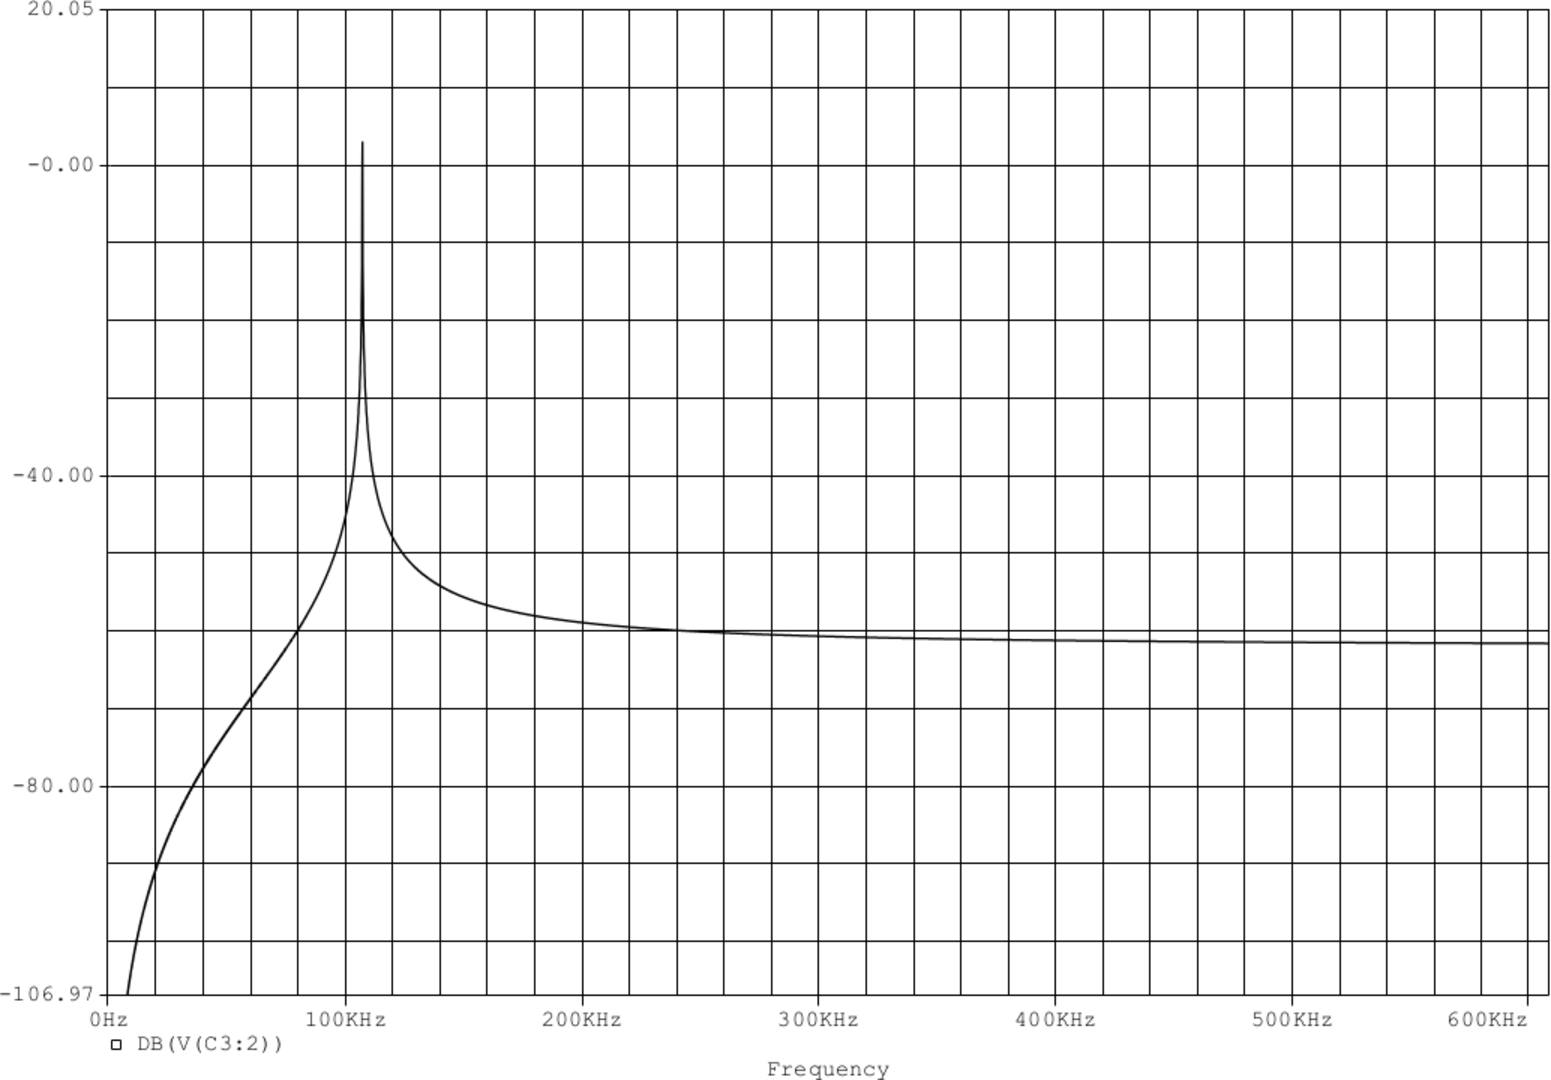
\includegraphics[scale=0.4]{Imagens/q_serie.pdf}
    \label{f_q_serie}
\end{figure}

Com base no gráfico da figura \ref{f_q_serie}, a largura de banda encontrada foi $BW_{3db} = 54.70 Hz$ e a frequência central $f_c = 106.98 kHz$. Assim, o fator de mérito do circuito é de
\[
Q_{load} = \frac{106.98*10^3}{54.70} = 1955,6
\]

Nota-se que o circuito, apesar de simples, possui um fator de mérito bastante elevado.\\

\subsection{Modulador a diodo}

\subsubsection{Filtro} 

Para o calculo do filtro, foi mantida a indutância de 1 mH, sendo assim, foi calculado o valor de $C_1$ de modo que a frequência central do filtro fosse de 100 kHz.
Então
\[
C_1 = \frac{1}{(2\pi f_c)^2 L } = \frac{1}{(2\pi 100*10^3 )^2 1*10^{-3}} = 2.53pF
\]

Foi, então, simulada a resposta em frequência do filtro, conforme mostra a figura \ref{f_filtro_diodo}, onde pode-se observar que a frequência central está, de fato, em 100kHz.

\begin{figure}[H]
    \centering
    \caption{Resposta em frequência para filtro do modulador a diodo.}
    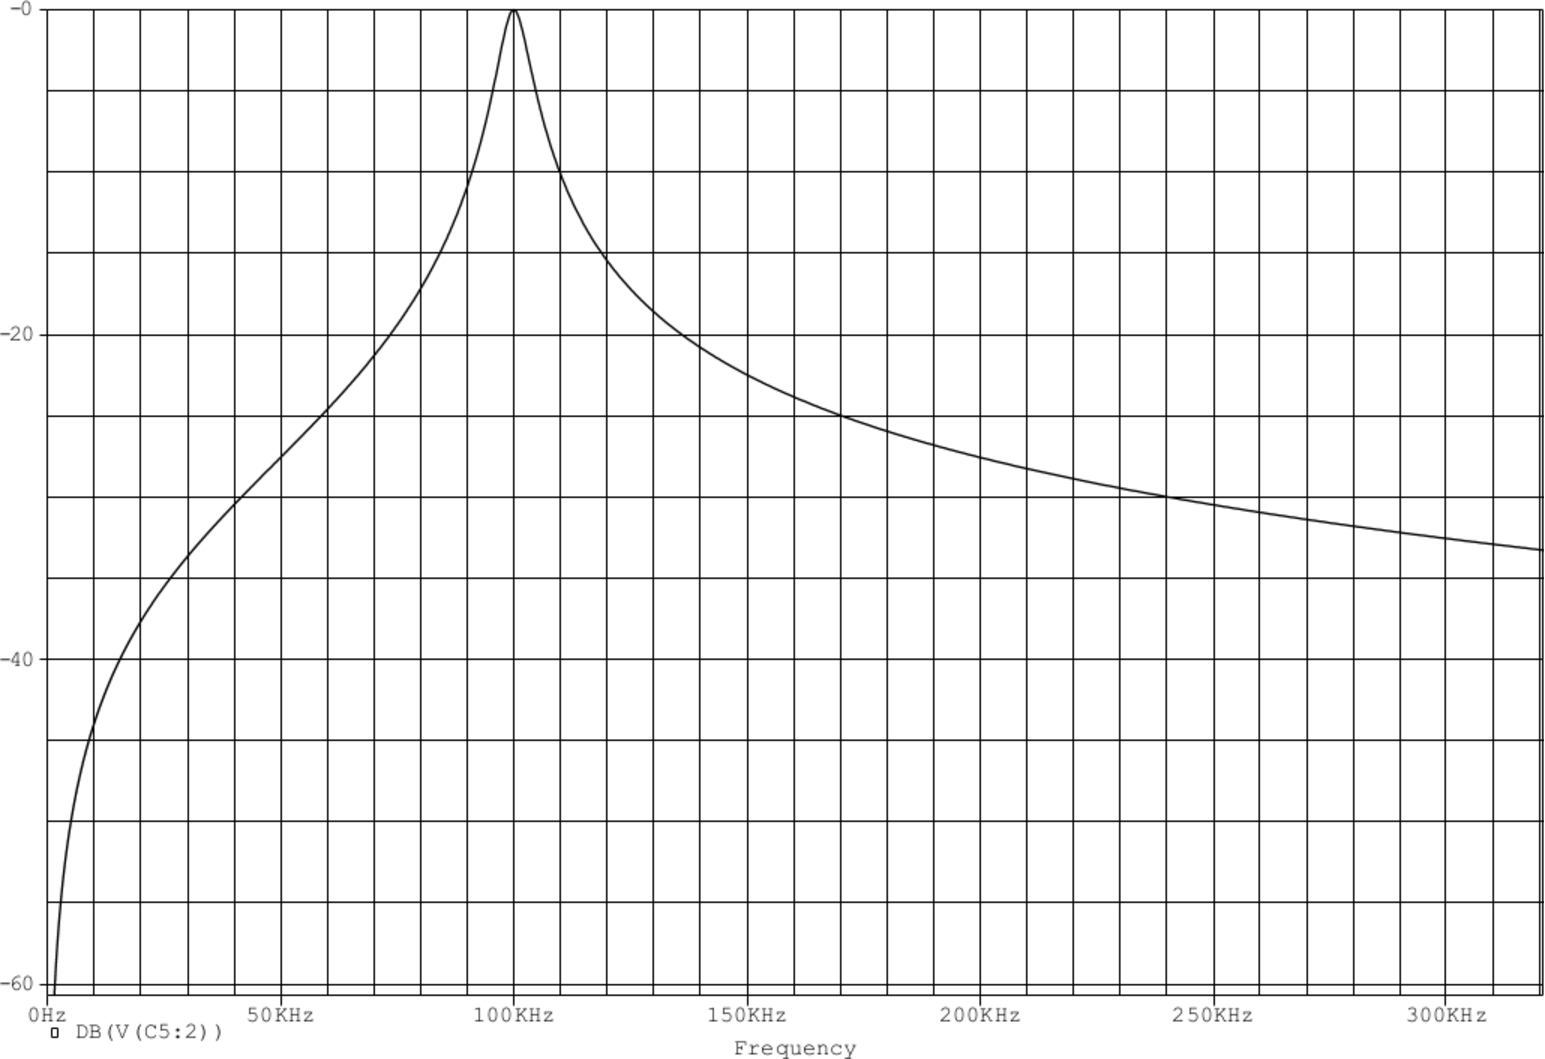
\includegraphics[scale=0.4]{Imagens/filtro_diodo.pdf}
    \label{f_filtro_diodo}
\end{figure}

\subsubsection{Sinal de saída}

Após a simulação, obtemos o sinal de saída mostrado na figura \ref{f_saida_diodo}. Pode-se observar um pequeno ceifamento do sinal de saída do modulador. Isso ocorre devido as características do diodo utilizado.

\begin{figure}[H]
    \centering
    \caption{Saída do modulador a diodo.}
    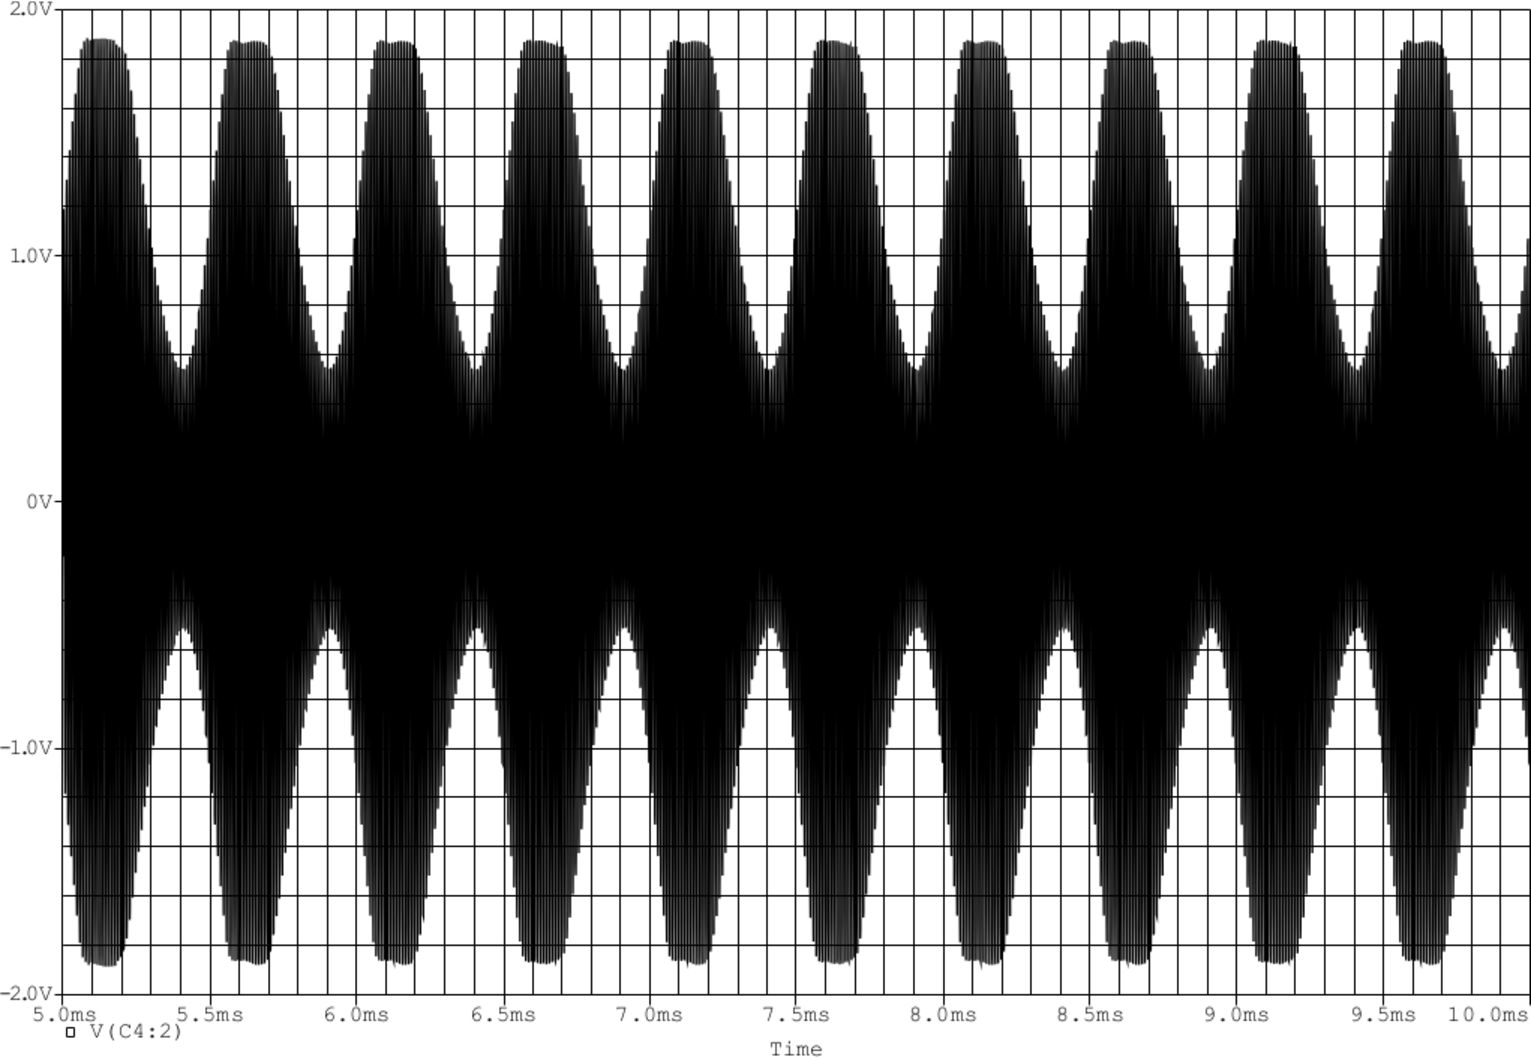
\includegraphics[scale=0.4]{Imagens/saida_diodo.pdf}
    \label{f_saida_diodo}
\end{figure}

Ao abrir a chave s1, foram observadas as formas de onda, na saída do modulador, das figuras \ref{f_saida_diodo_s1_antes} e \ref{f_saida_diodo_s1_depois}, antes e depois do diodo $D_1$, respectivamente.

\begin{figure}[H]
    \centering
    \caption{Saída do modulador a diodo com a chave s1 aberta (antes do diodo $D_1$).}
    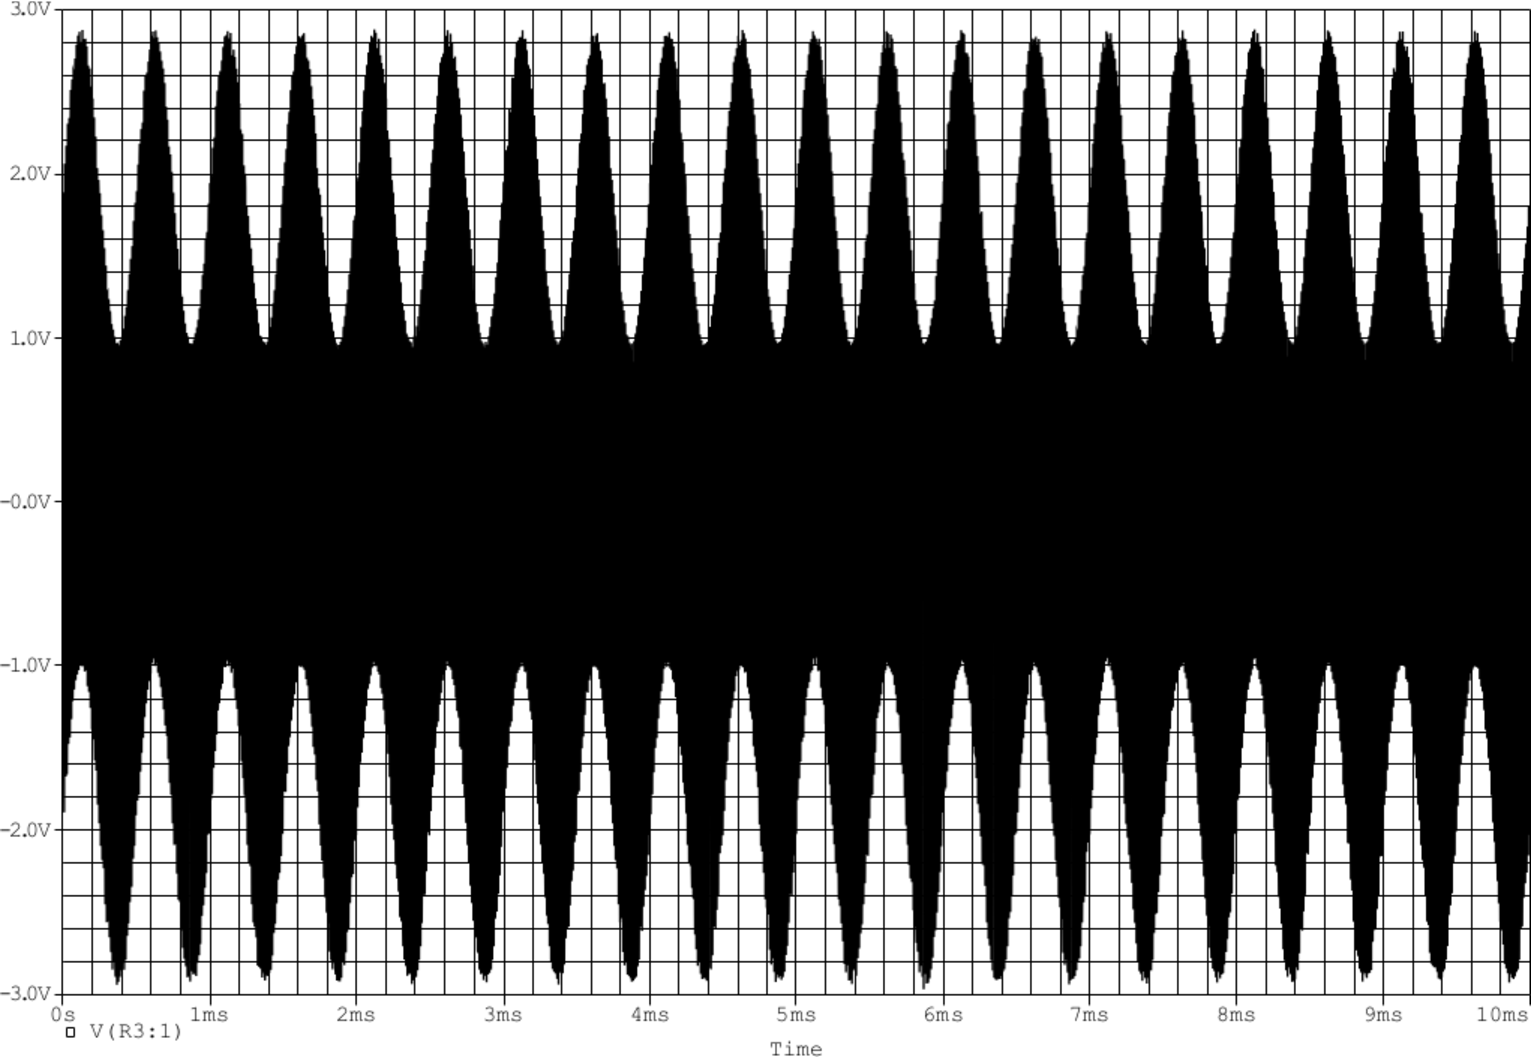
\includegraphics[scale=0.4]{Imagens/saida_diodo_s1_antes.pdf}
    \label{f_saida_diodo_s1_antes}
\end{figure}

\begin{figure}[H]
    \centering
    \caption{Saída do modulador a diodo com a chave s1 aberta (após o diodo $D_1$).}
    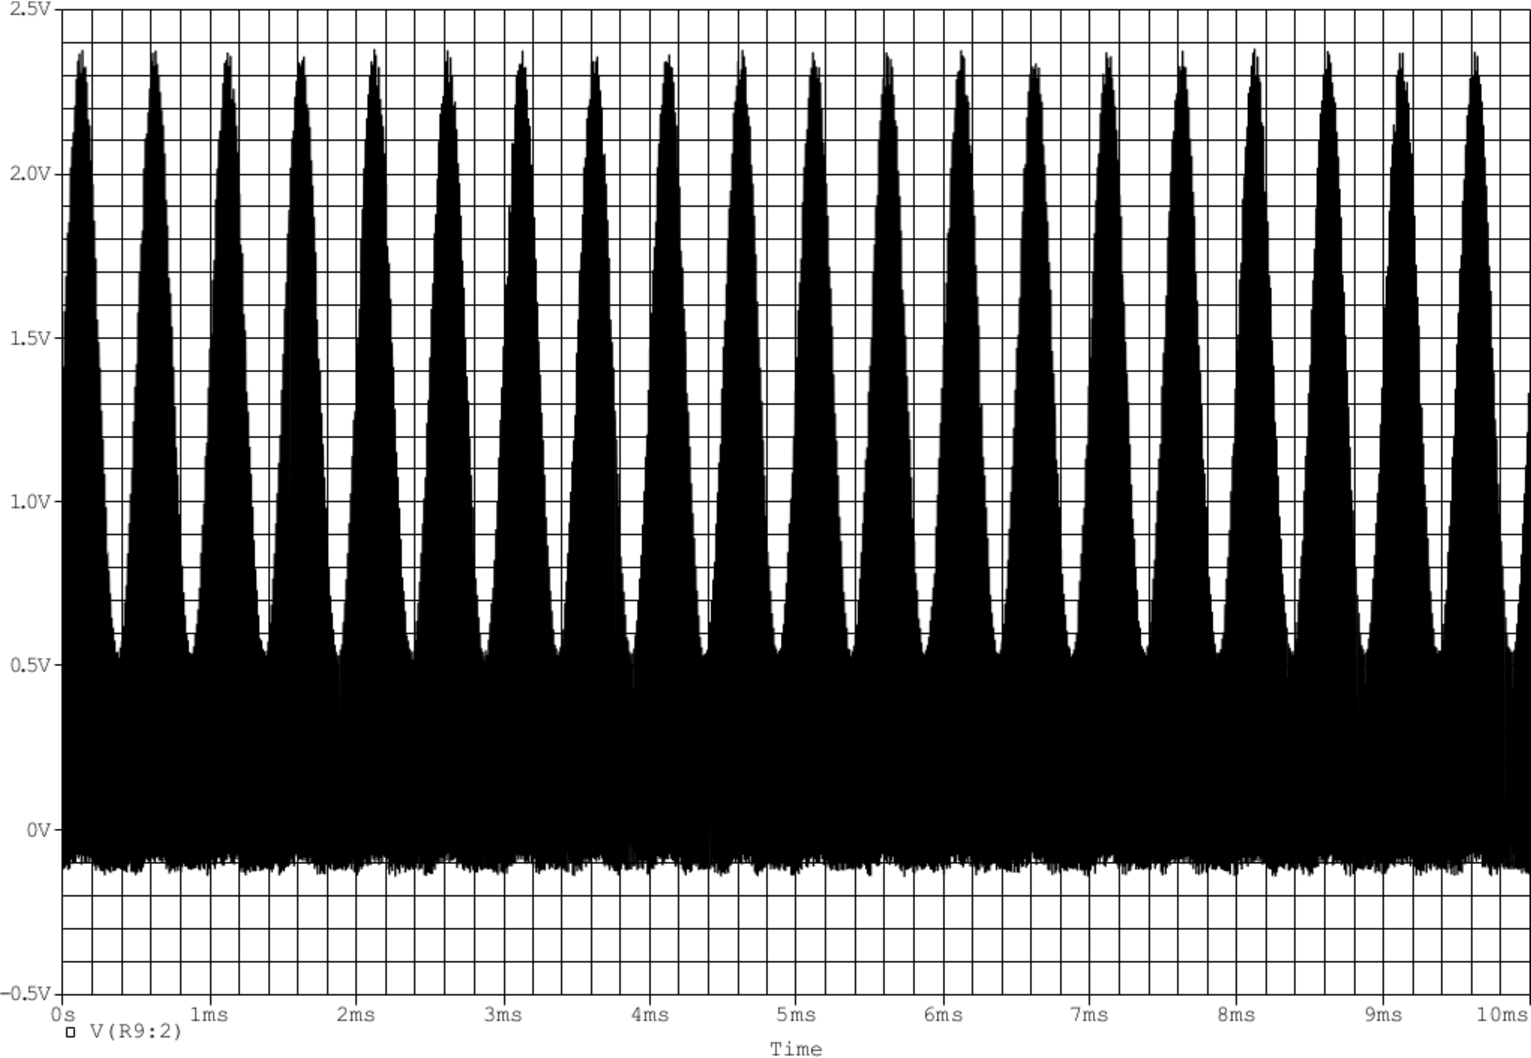
\includegraphics[scale=0.4]{Imagens/saida_diodo_s1_depois.pdf}
    \label{f_saida_diodo_s1_depois}
\end{figure}

\subsubsection{Índice de modulação}
O índice de modulação calculado a partir do sinal da figura \ref{f_saida_diodo}, utilizando o método 1, foi de $\gamma = 0.6462$.

A figura \ref{f_trapezio_diodo} mostra o resultado do método do trapézio (método 2). Como pode ser observado, a curva não é linear em amplitude, devido as distorções causadas pelo diodo. Sendo assim, não foi possível a obtenção do índice de modulação, de forma precisa, a partir deste método.

\begin{figure}[H]
    \centering
    \caption{Método do trapézio para modulador a diodo.}
    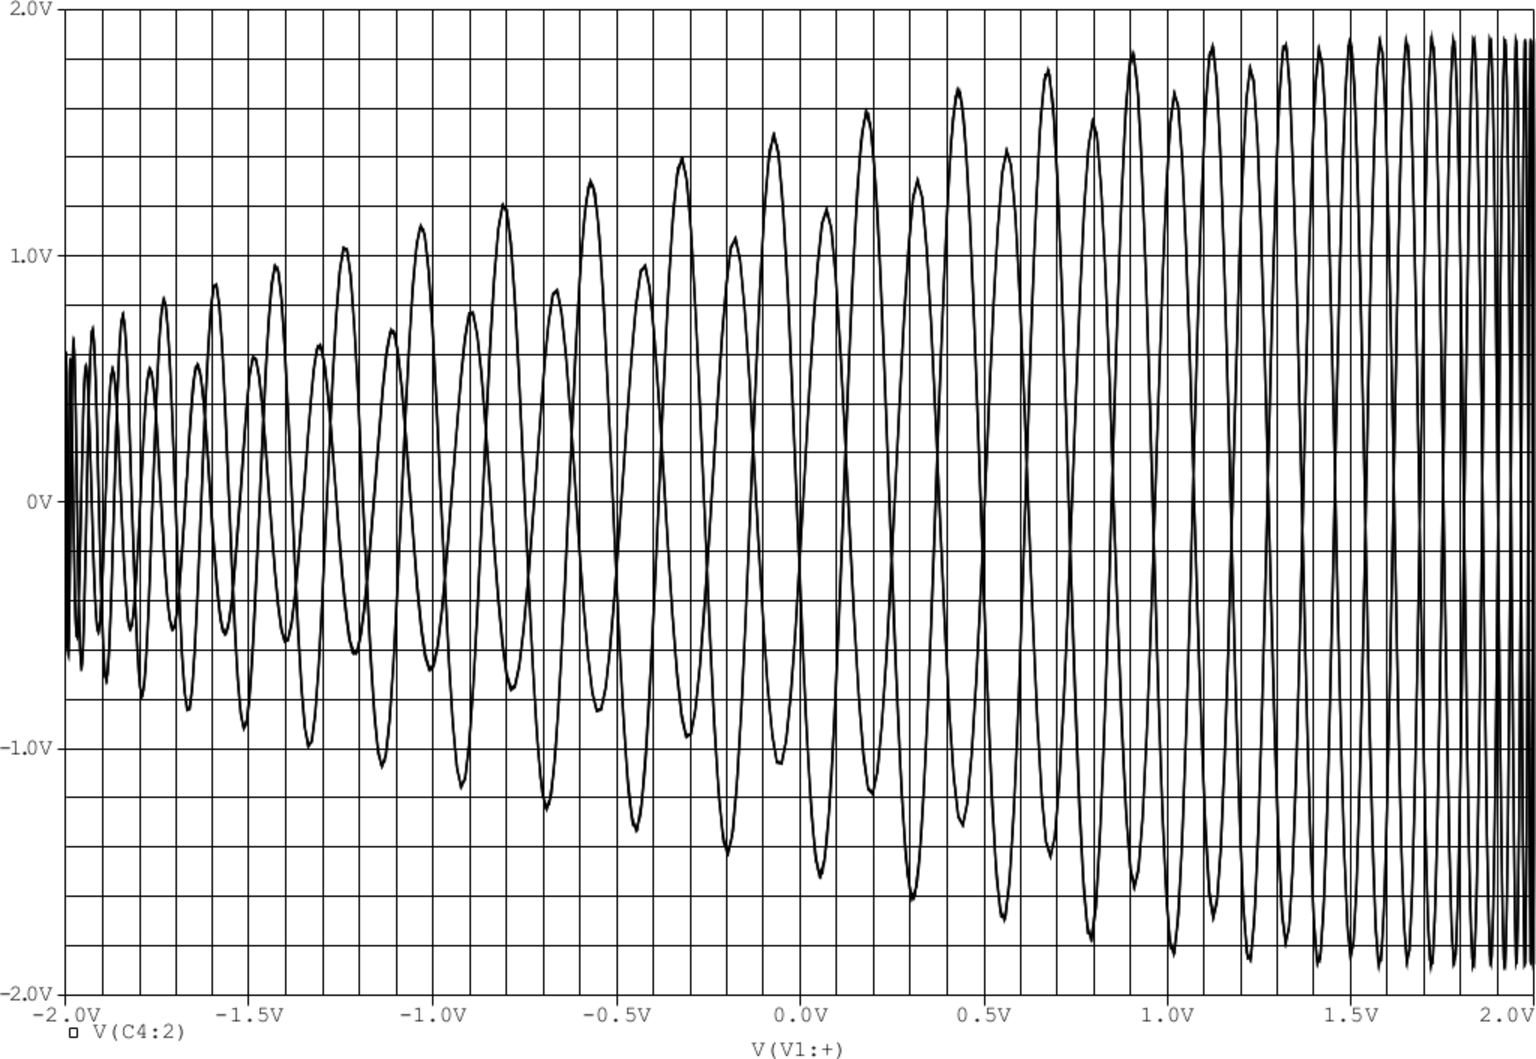
\includegraphics[scale=0.4]{Imagens/trapezio_diodo.pdf}
    \label{f_trapezio_diodo}
\end{figure}

\subsubsection{Espectro do sinal modulado}
A figura \ref{f_fft_diodo} mostra o espectro do sinal de saída do modulador a diodo. Observa-se, novamente, a presença da portadora e das duas raias laterais do sinal AM modulado, que são as características da modulação AM/DSB. Porém, é notável a presença de outras componentes harmônicas no sinal.

\begin{figure}[H]
    \centering
    \caption{Espectro do sinal modulado com modulador a diodo.}
    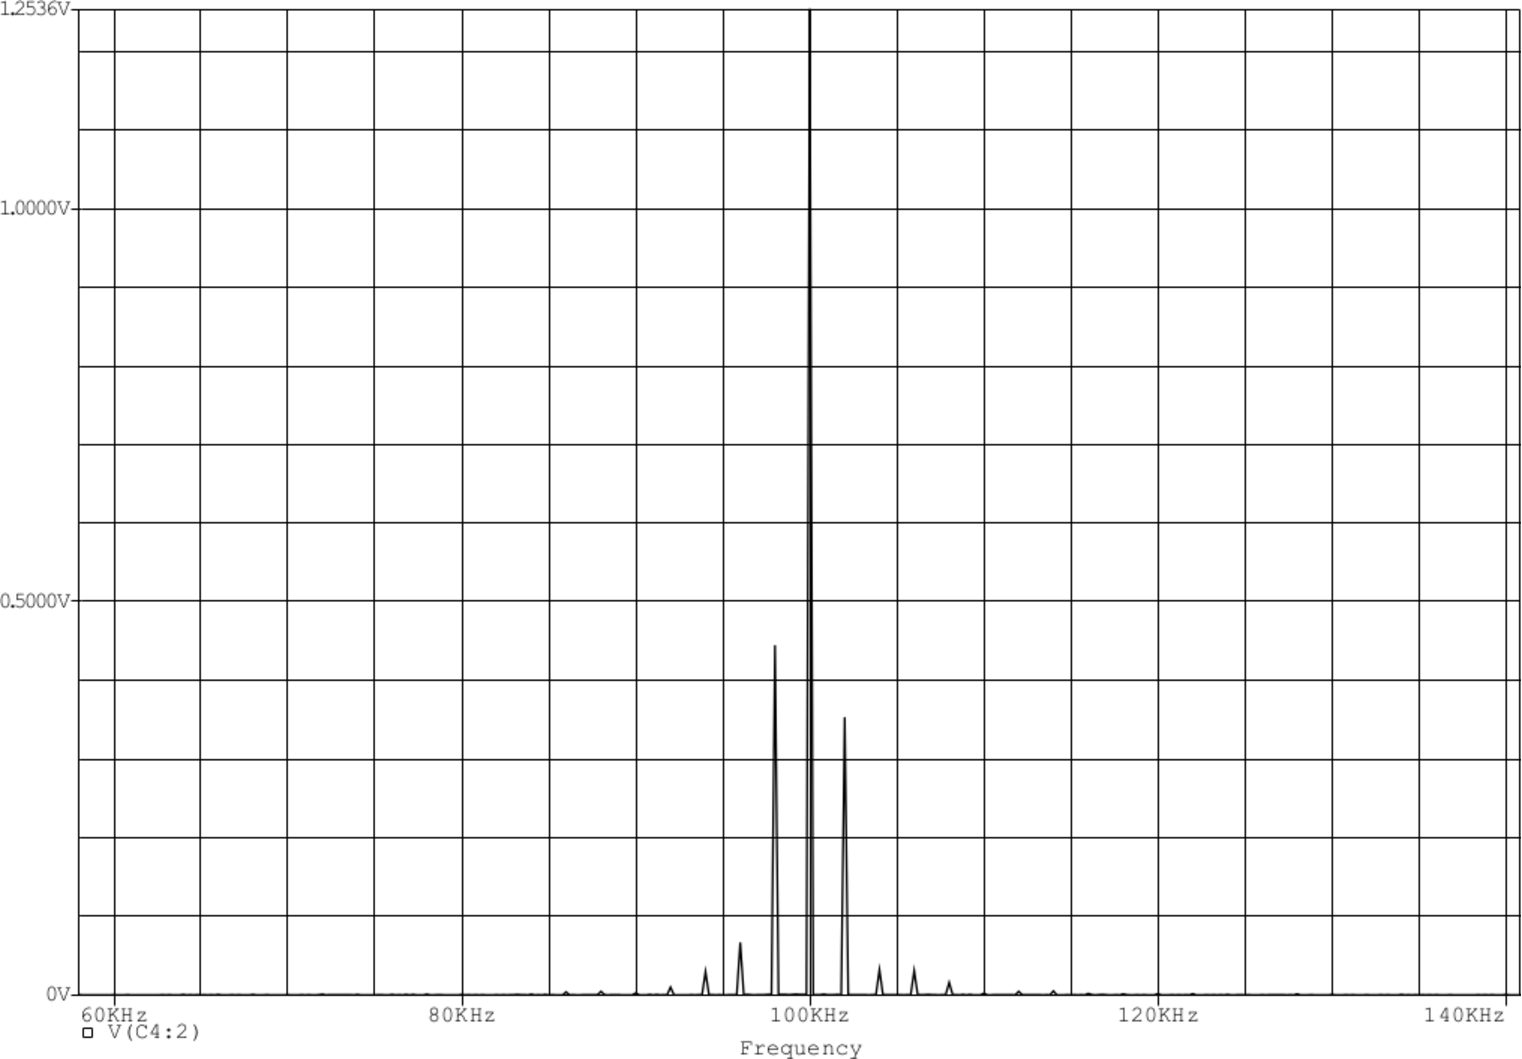
\includegraphics[scale=0.4]{Imagens/fft_diodo.pdf}
    \label{f_fft_diodo}
\end{figure}

\subsubsection{Fator de mérito}
O gráfico da resposta em frequência do modulador a diodo é apresentado na figura \ref{f_q_diodo}, de onde podemos extrair o valor de $BW_{3dc} = 2.83 kHz$ e $f_c = 99.54 kHz$. Assim, o fator de mérito do circuito é

\[
Q_{diodo} = \frac{99.54*10^3}{2.8*10^3} = 35.14. 
\]


\begin{figure}[H]
    \centering
    \caption{Resposta em frequência do modulador a diodo.}
    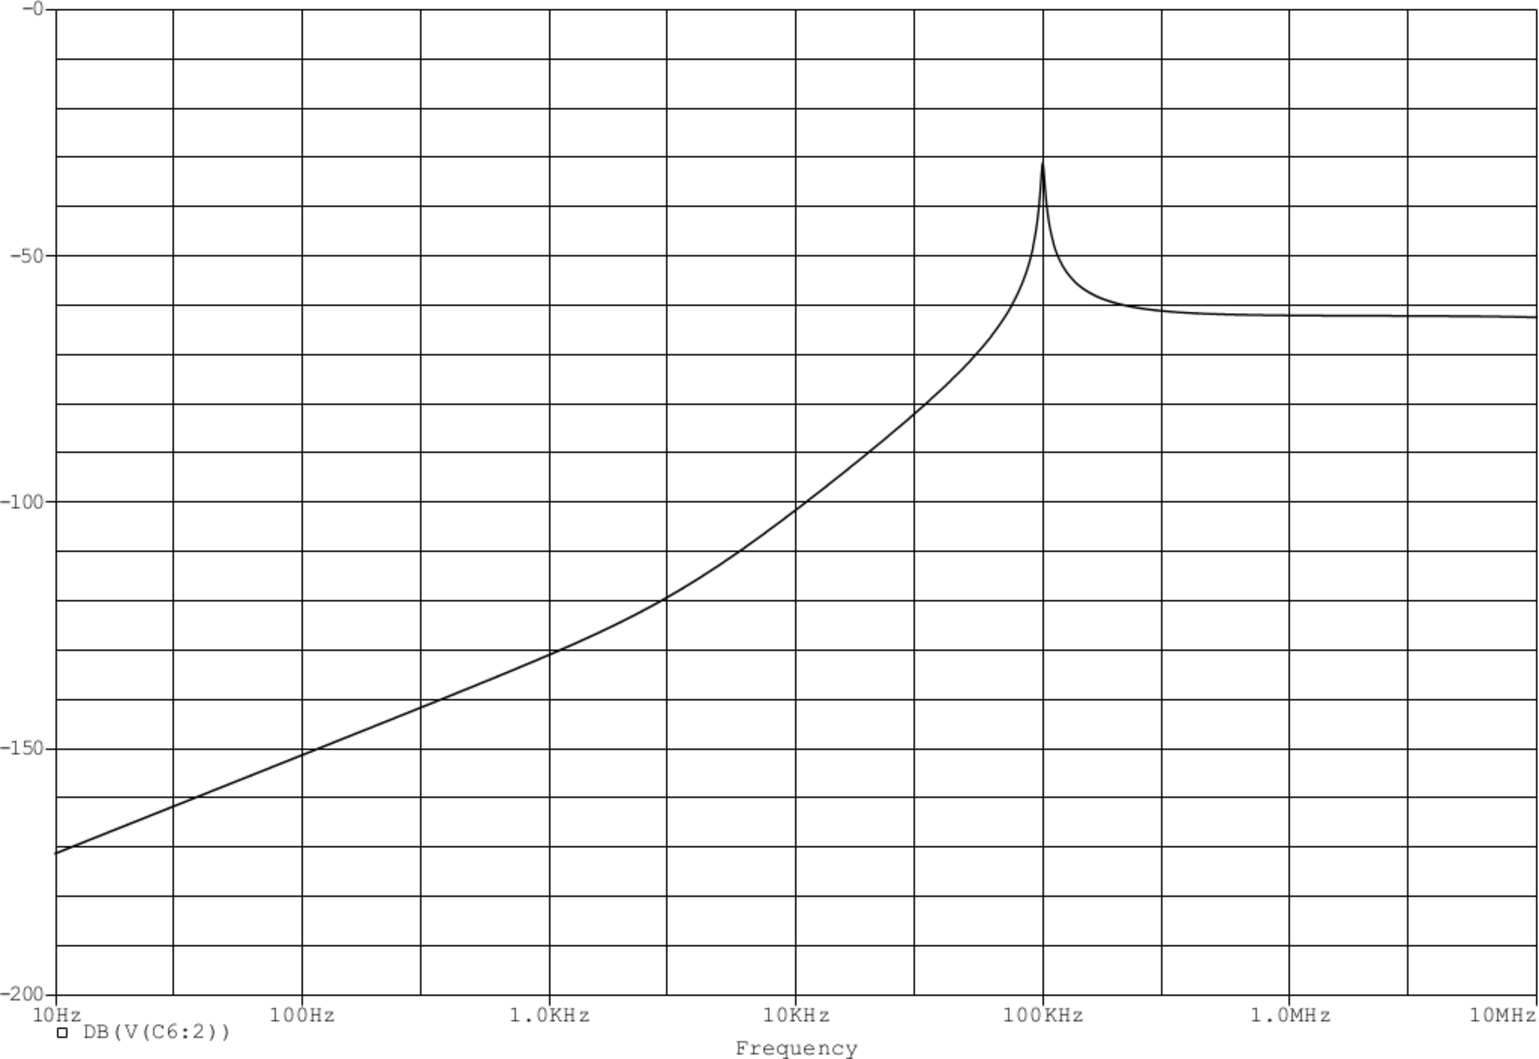
\includegraphics[scale=0.4]{Imagens/q_diodo.pdf}
    \label{f_q_diodo}
\end{figure}


